\documentclass[twocolumn,a4j]{jsarticle}
\setlength{\topmargin}{-20.4cm}
\setlength{\oddsidemargin}{-10.4mm}
\setlength{\evensidemargin}{-10.4mm}
\setlength{\textwidth}{18cm}
\setlength{\textheight}{26cm}

\usepackage[top=15truemm,bottom=20truemm,left=20truemm,right=20truemm]{geometry}
\usepackage[latin1]{inputenc}
\usepackage{amsmath}
\usepackage{amsfonts}
\usepackage{amssymb}
\usepackage[dvipdfmx]{graphicx}
\usepackage[hang,small,bf]{caption}
\usepackage[subrefformat=parens]{subcaption}
\usepackage[dvipdfmx]{color}
\usepackage{listings}
\usepackage{listings,jvlisting}
\usepackage{geometry}
\usepackage{framed}
\usepackage[dvipdfmx]{hyperref}
\usepackage{ascmac}
\usepackage{enumerate}
\usepackage{tabularx}
\usepackage{cancel}
\usepackage{scalefnt}
\usepackage{overcite}
\usepackage{otf}
\usepackage{multicol}
\usepackage[geometry]{ifsym}
\usepackage{array}

\renewcommand{\figurename}{Fig.}
\renewcommand{\tablename}{Table }

\lstset{
basicstyle={\ttfamily},
identifierstyle={\small},
commentstyle={\smallitshape},
keywordstyle={\small\bfseries},
ndkeywordstyle={\small},
stringstyle={\small\ttfamily},
frame={tb},
breaklines=true,
columns=[l]{fullflexible},
xrightmargin=0zw,
xleftmargin=3zw,
numberstyle={\scriptsize},
stepnumber=1,
numbersep=1zw,
lineskip=-0.5ex
}

% キャプション後ろのダブルコロンを消す
\makeatletter
\long\def\@makecaption#1#2{%
  \vskip\abovecaptionskip
  \iftdir\sbox\@tempboxa{#1\hskip1zw#2}%
    \else\sbox\@tempboxa{#1 #2}%
  \fi
  \ifdim \wd\@tempboxa >\hsize
    \iftdir #1\hskip1zw#2\relax\par
      \else #1 #2\relax\par\fi
  \else
    \global \@minipagefalse
    \hbox to\hsize{\hfil\box\@tempboxa\hfil}%
  \fi
  \vskip\belowcaptionskip}
\makeatother

% タイトル
\makeatletter
\def\@maketitle
{
\begin{center}
{\LARGE \@title \par}
\end{center}
\begin{flushright}
{\large \@date 報告書 No.41}\\
{\large M2 \@author}
\end{flushright}
\par\vskip 1.5em
}
\makeatother

\author{来代 勝胤}
\title{令和4年度 11月 第3週 報告書}
\date{2022/11/21}

\begin{document}
\columnseprule=0.1mm
\maketitle

\section*{報告内容}
\begin{enumerate}[1.]
  \item 数値シミュレーションの修正
  \item 来週の予定
\end{enumerate}

\section{数値シミュレーションの修正}
数値シミュレーションの解析について,先週の結果に基づいて修正を行った.
今回は,三角翼後流部の検査体積を 300 mm から 800 mm に大きくして解析を行い,
同様に速度場を計算した.

\begin{figure}[htbp]
  \centering
  {
    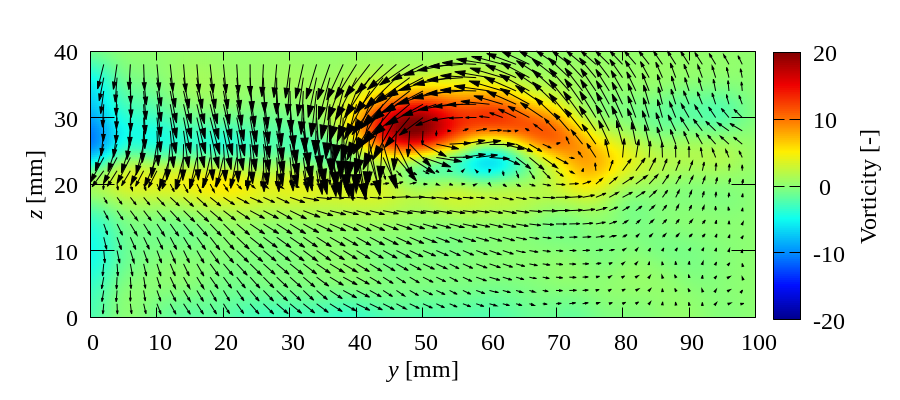
\includegraphics[keepaspectratio, width=80mm]{../images/Simulation/Compare/experiment_x=0.png}
    \subcaption{Experiment}
    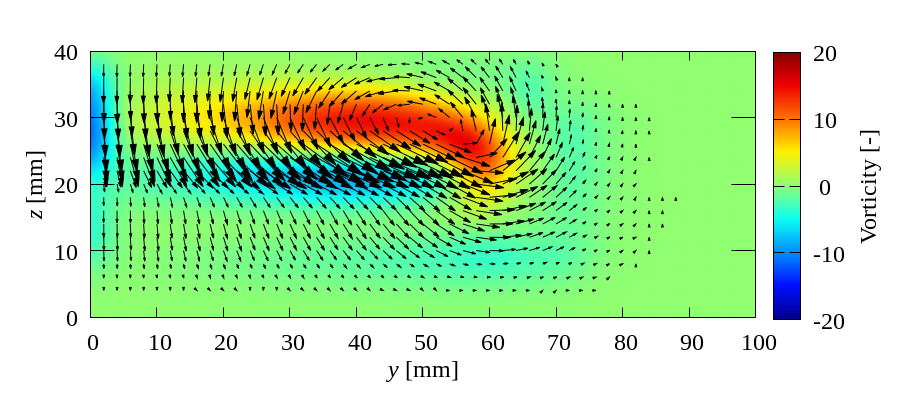
\includegraphics[keepaspectratio, width=80mm]{../images/Simulation/Compare/simulation_x=0.png}
    \subcaption{Previous simulation}
    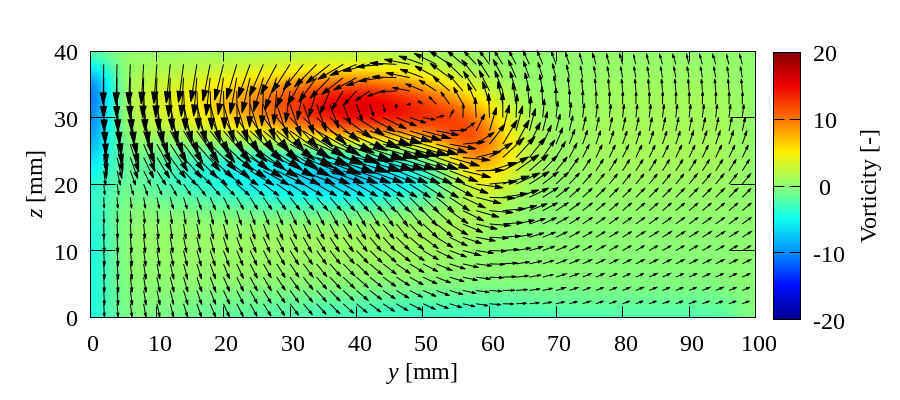
\includegraphics[keepaspectratio, width=80mm]{../images/Simulation/Compare/simulation2_x=0.png}
    \subcaption{Fixed simulation}
  }
  \caption{Delta wing :$x=0$}
\end{figure}

\newpage
\begin{figure}[htbp]
  \centering
  {
    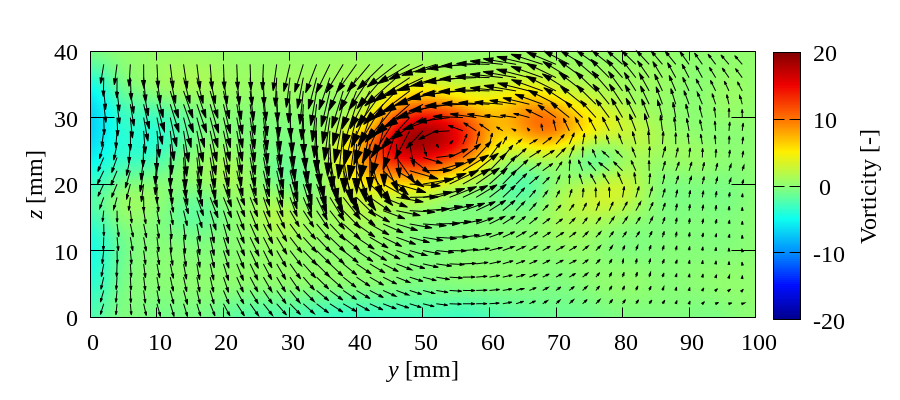
\includegraphics[keepaspectratio, width=80mm]{../images/Simulation/Compare/experiment_x=20.png}
    \subcaption{Experiment}
    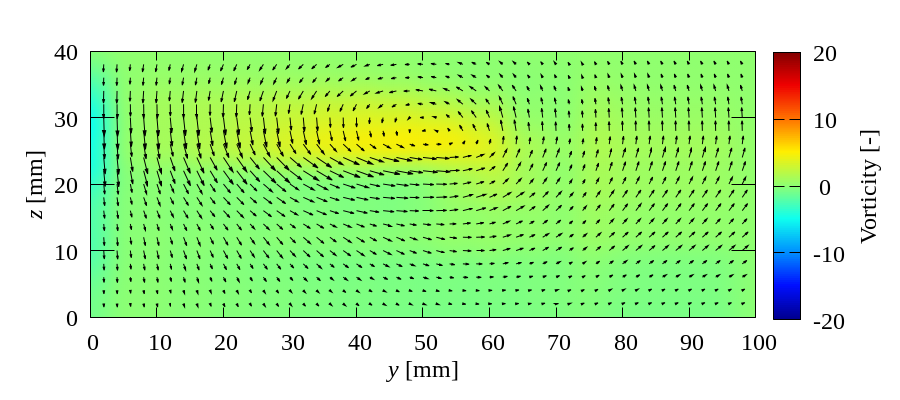
\includegraphics[keepaspectratio, width=80mm]{../images/Simulation/Compare/simulation_x=20.png}
    \subcaption{Previous simulation}
    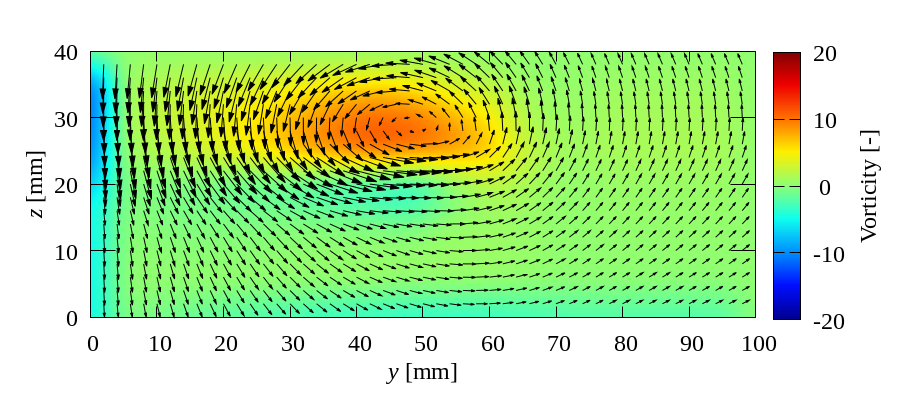
\includegraphics[keepaspectratio, width=80mm]{../images/Simulation/Compare/simulation2_x=20.png}
    \subcaption{Fixed simulation}
  }
  \caption{Delta wing :$x=20$}
\end{figure}

\newpage
\begin{figure}[htbp]
  \centering
  {
    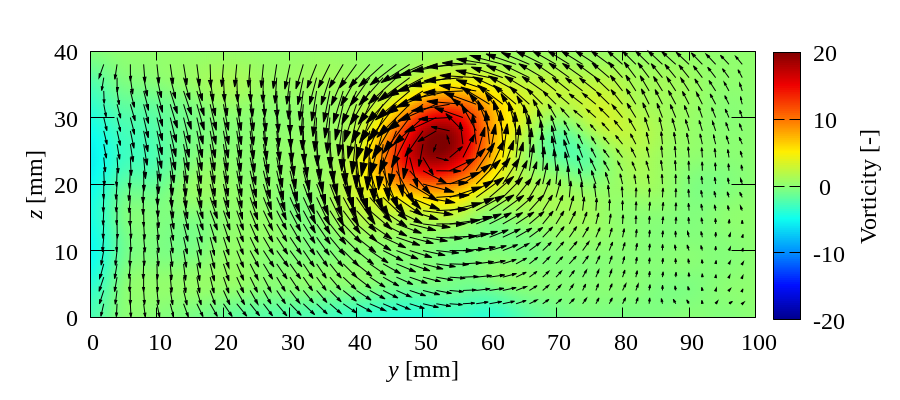
\includegraphics[keepaspectratio, width=80mm]{../images/Simulation/Compare/experiment_x=40.png}
    \subcaption{Experiment}
    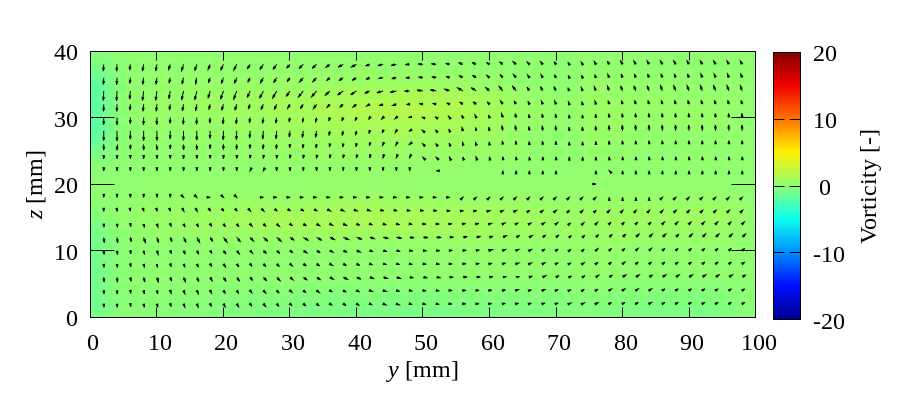
\includegraphics[keepaspectratio, width=80mm]{../images/Simulation/Compare/simulation_x=40.png}
    \subcaption{Previous simulation}
    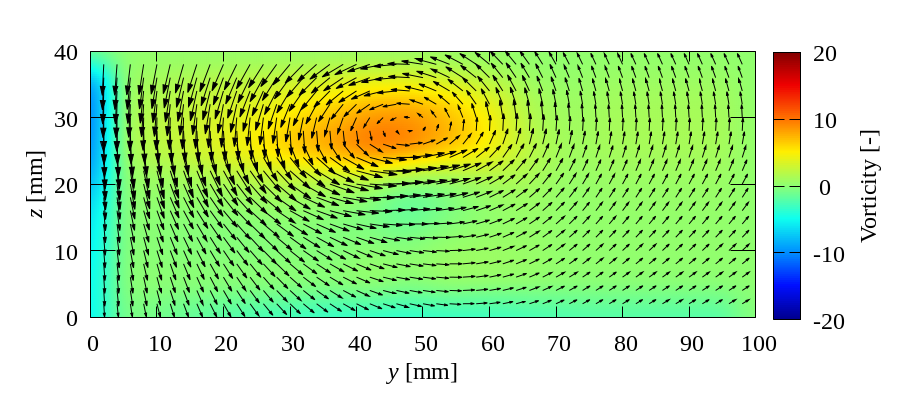
\includegraphics[keepaspectratio, width=80mm]{../images/Simulation/Compare/simulation2_x=40.png}
    \subcaption{Fixed simulation}
  }
  \caption{Delta wing :$x=40$}
\end{figure}


\section{来週の予定}
\begin{itemize}
  \item 数値シミュレーションデータの解析
  \item 共同研究報告書の作成
\end{itemize}

\end{document}